\subsection{Community Support}

{
\setbeamertemplate{background canvas}{\tikz[remember picture]\node[opacity=0.7] at (current page.center) {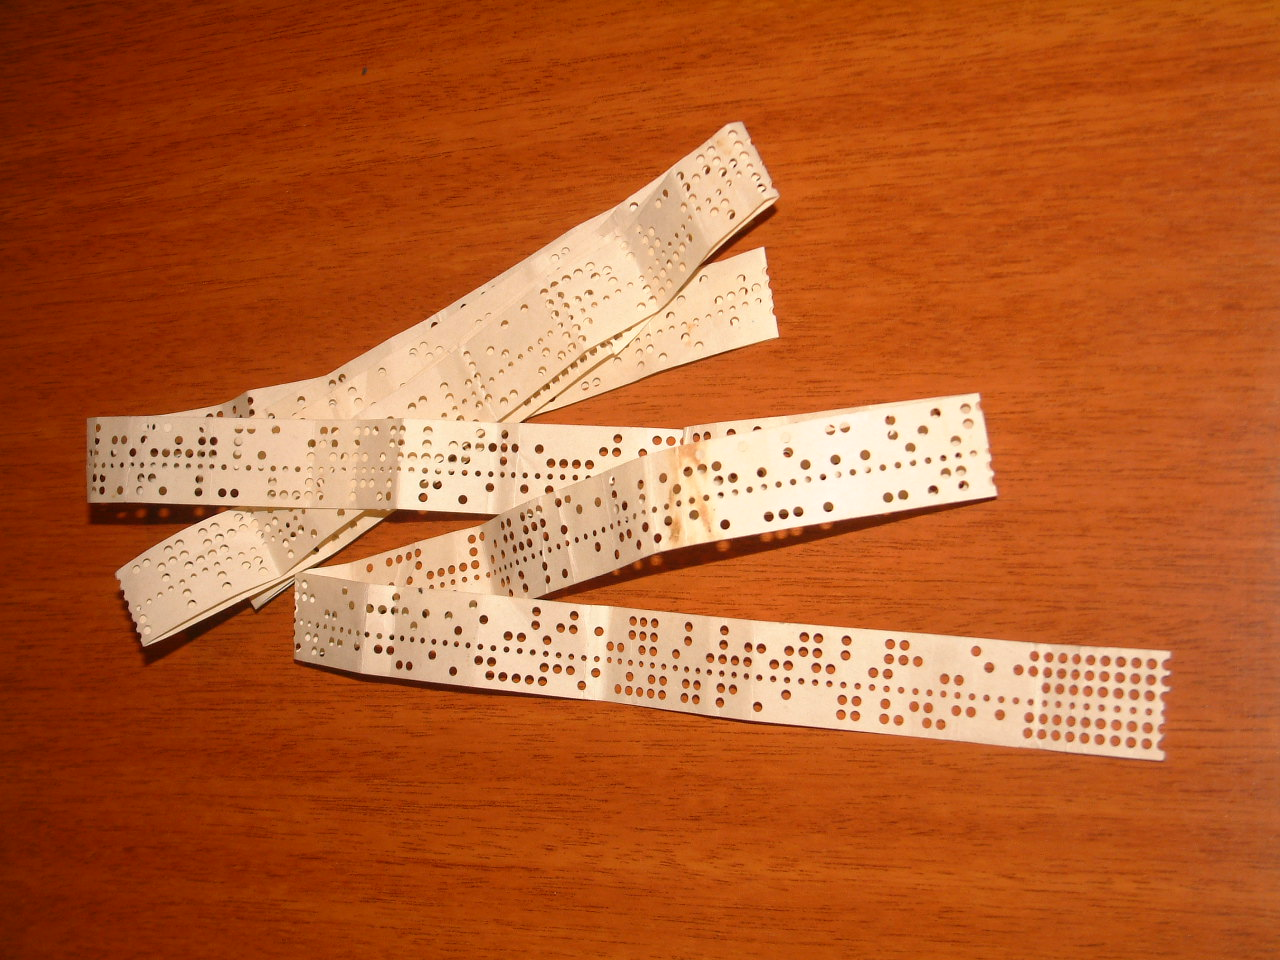
\includegraphics[height=1.05\textheight,keepaspectratio]{nontex/illustrations/baudotTape.jpg}};}
\begin{frame}
\frametitle{How Does The Community Prefer To Represent Regexes?}
\begin{block}{\begin{Large}Knowledge Of Community Standards Is Missing\end{Large}}
\begin{itemize}
\item \begin{large}programmers probably choose the best representation\end{large}
\item \begin{large}conformance to community standards may ease comprehension\end{large}
\end{itemize}
\end{block}
\end{frame}
}
\note[itemize]{
    \item https://i.ytimg.com/vi/Gt-5lS9hJFA/hqdefault.jpg
        \item cite that fact!
}

%------------------------------------------------


\begin{frame}
\frametitle{Node Membership Counts}
\begin{adjustbox}{width=\textwidth}
\begin{tabular}
{lll@{}rrrr}
\textbf{Node} & \textbf{Description} & \textbf{Example} & \textbf{NProjects} & \% \textbf{Projects} \\ \textbf{NRegexes} & \% \textbf{Regexes} &
\toprule[0.16em]
%corpusProjectIDs.size(): 1544
C1 & CCC using RNG & \begin{minipage}{1.2in}\begin{verbatim}^[1-9][0-9]*$\end{verbatim}\end{minipage} & 810 & 52.5\%\\ 2,479 & 18.2\% &
C2 & CCC listing all chars & \begin{minipage}{1.2in}\begin{verbatim}[aeiouy]\end{verbatim}\end{minipage} & 715 & 46.3\%\\ 1,903 & 14.0\% &
C3 & any NCCC & \begin{minipage}{1.2in}\begin{verbatim}[^A-Za-z0-9.]+\end{verbatim}\end{minipage} & 776 & 50.3\%\\ 1,935 & 14.2\% &
C4 & CCC using defaults & \begin{minipage}{1.2in}\begin{verbatim}[-+\d.]\end{verbatim}\end{minipage} & 414 & 26.8\%\\ 840 & 6.2\% &
C5 & CCC as an OR & \begin{minipage}{1.2in}\begin{verbatim}(@|<|>|-|!)\end{verbatim}\end{minipage} & 239 & 15.5\%\\ 245 & 1.8\% &
\midrule
D1 & repetition like \{M,N\}& \begin{minipage}{1.2in}\begin{verbatim}^x{1,4}$\end{verbatim}\end{minipage} & 234 & 15.2\%\\ 346 & 2.5\% &
D2 & zero-or-one repetition & \begin{minipage}{1.2in}\begin{verbatim}^http(s)?://\end{verbatim}\end{minipage} & 646 & 41.8\%\\ 1,871 & 13.8\% &
D3 & repetition using OR & \begin{minipage}{1.2in}\begin{verbatim}^(Q|QQ)\<(.+)\>$\end{verbatim}\end{minipage} & 27 & 1.7\%\\ 10 & .1\% &
\midrule
T1 & not in T2, T3 or T4 & \begin{minipage}{1.2in}\begin{verbatim}get_tag\end{verbatim}\end{minipage} & 1,485 & 96.2\%\\ 12,482 & 91.8\% &
T2 & has HEX like \verb!\xF5! & \begin{minipage}{1.2in}\begin{verbatim}[\x80-\xff]\end{verbatim}\end{minipage} & 243 & 15.7\%\\ 479 & 3.5\% &
T3 & wrapped chars like [\$] & \begin{minipage}{1.2in}\begin{verbatim}([*]|[:])\end{verbatim}\end{minipage} & 268 & 17.4\%\\ 307 & 2.3\% &
T4 & has OCT like \verb!\0177! & \begin{minipage}{1.2in}\begin{verbatim}[\041-\176]+:$\end{verbatim}\end{minipage} & 37 & 2.4\%\\ 14 & .1\% &
\midrule
L1 & repetition like \{M,\} & \begin{minipage}{1.2in}\begin{verbatim}(DN)[0-9]{4,}\end{verbatim}\end{minipage} & 166 & 10.8\%\\ 91 & .7\% &
L2 & kleene star repetition & \begin{minipage}{1.2in}\begin{verbatim}\s*(#.*)?$\end{verbatim}\end{minipage} & 1,097 & 71.0\%\\ 6,017 & 44.3\% &
L3 & additional repetition& \begin{minipage}{1.2in}\begin{verbatim}[A-Z][a-z]+\end{verbatim}\end{minipage} & 1,207 & 78.2\%\\ 6,003 & 44.1\% &
\midrule
S1 & repetition like \{M\} & \begin{minipage}{1.2in}\begin{verbatim}^[a-f0-9]{40}$\end{verbatim}\end{minipage} & 340 & 22.0\%\\ 581 & 4.3\% &
S2 & sequential repetition & \begin{minipage}{1.2in}\begin{verbatim}ff:ff:ff:ff:ff:ff\end{verbatim}\end{minipage} & 861 & 55.8\%\\ 3,378 & 24.8\% &
S3 & repetition like \{M,M\} & \begin{minipage}{1.2in}\begin{verbatim}U[\dA-F]{5,5}\end{verbatim}\end{minipage} & 32 & 2.1\%\\ 27 & .2\% &
\bottomrule[0.13em]
\end{tabular}
\end{adjustbox}

\end{frame}
\note[itemize]{
    \item pt 1
    \item pt 2
}

%------------------------------------------------
